% Contribution chapter no. 2 (TOP20 pick 2, id Z-BAO-P23) -- English translation of chapters/c02.tex
% Sources: papers/certified_desi_h0/ (certified_desi_h0.tex, publication_meta.json),
% results/certified_numerics/P2_likelihood/ and P3_h0/ (result.json, verification.md), TOP20.json.
\chapter[A tension written as an inequality]{A famous tension in cosmology, written as a verified inequality}
\reference{Published on 10 October 2026.\\ doi:10.5281/\\zenodo.23284020}

\section*{The idea in one picture}

\begin{analogie}
Imagine we want to prove that a radio picks up no station beyond the 73 mark on the dial. We cannot listen at
infinitely many positions of the knob. So we cut the dial into bands, and for each band a notary signs a statement:
``throughout this band, the signal stays below such-and-such a level.'' When all the bands are signed, the whole dial
is covered, with no gap.

\emph{Where the picture stops:} here, ``no station'' means ``the data fit much worse'', not ``impossible''; and the
statement holds only for the radio we described, that is, for the chosen model.
\end{analogie}

\section*{What was done}

The universe is expanding, and its present rate of expansion is called $H_0$. Two families of measurements disagree
on its value: this is the ``Hubble tension''. Nearby measurements, made with a ladder of distances, give about
73\,km/s per megaparsec. Measurements of the standard ruler from the previous chapter, combined with what the first
minutes of the universe tell us about the light elements, give about 68.5 (DESI publishes $68.51\pm0.58$).

The work turns two known statements into theorems checked by the machine. The first: with DESI's measurements alone,
a matter share $\Omega_m$ between 0 and 0.255, or between 0.35 and 1, fits much worse than the best fit, whatever the
size of the ruler. The second: with the light elements added, every value $H_0\ge73$ fits much worse, whatever the
matter share and the density of baryons. ``Much worse'' has a precise meaning: a mismatch score, written $\chi^2$,
exceeds by more than 25 that of a certified reference point ($\chi^2\le10.2897$).

\begin{encadre}
\textbf{To do with a pencil: covering infinitely many values at once.} The size of the ruler is an unknown $t$ that
can take any value. The score has the form $c-Bt+At^2$. Take $3-2t+t^2$. Rewrite it as $(t-1)^2+2$: a square is never
negative, so the score is at least $2$ \emph{for every} $t$. Check: $t=0$ gives $3$, $t=1$ gives $2$, $t=3$ gives
$6$. In general, if $A>0$, the score is at least $c-B^2/(4A)$; here $3-4/4=2$. A single inequality settles infinitely
many cases.

\textbf{The threshold.} $35.2897-10.2897=25=5^2$: this is the conventional gap called ``5 sigmas'' when one looks at a
single parameter (about 4.3 sigmas if one reads the joint region of the three parameters).
\end{encadre}

To cover all the values of the parameters, the space is cut into slices and boxes, like the radio dial: 29 slices for
the matter share, 89 boxes for the question of $H_0$. On each box, an interval evaluator, proved correct once and for
all, bounds the score with exact fractions. Figure~\ref{fig:c02} shows the same thing computed in the ordinary way:
the curve crosses the threshold 25 at about $H_0\approx71.6$, and the gap from the best point is about $54.6$ at $H_0=73$. The value 73 is
therefore a reference value, chosen in advance; it is not the edge of the excluded region.

\begin{figure}[htbp]
\centering
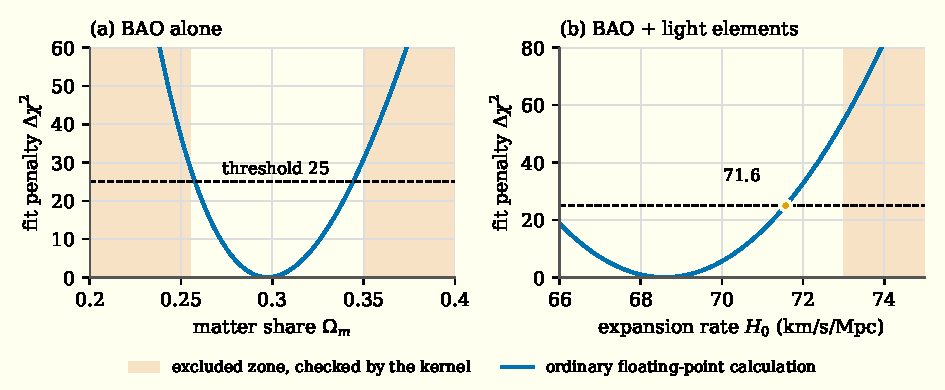
\includegraphics[width=\linewidth]{figures/c02_profils}
\caption{Curves: ordinary floating-point calculation recomputed from the data (level X). Shaded zones: what the
kernel verified. (a) Matter share, DESI alone. (b) Expansion rate, DESI and light elements.}
\label{fig:c02}
\end{figure}

\section*{How we made sure it is not wrong}

\niveau{As} \emph{The judge looked, without a replay.} The judge is Lean, a program that checks every step of a proof.
The bounds on logarithms and exponentials come from results already proved in its mathematical library, and only the
three basic assumptions accepted everywhere appear. These files are not in the full replay of 26 October: hence
``without a replay''.

The tests designed to fail did fail. A copy of the data in which one value is shifted by 10 standard deviations makes
the certified score jump to $[122.69\,;\,122.76]$. A slice that contains the best fit is not excluded. Above all, an
independent checker rebuilt the 173 modules of the final theorem and found that the proof breaks if a threshold of 65
is requested instead of $35.29$: this is as it should be, because the statement would become false (the score is
$64.91$ at $H_0=73$).

A failure was also published. The slicing fixed \emph{before} the calculation excluded only 8 slices out of 19; the
announced prediction was not met. A finer slicing, decided after the fact, was declared as such. Two independent
checks by AI agents (including the rebuilding of 3 of the 29 slices) gave a favourable opinion with corrections. No
human has redone these calculations.

\section*{What this does not say}

\begin{limite}
\begin{itemize}
\item This is a certified version of a tension already known from ordinary statistics, not a new measurement.
\item The model is simplified: a flat universe, radiation neglected, one fitting formula for the size of the ruler,
errors assumed to follow a bell curve (Gaussian).
\item Nothing here says where the tension comes from, or which of the two families of measurements is right.
\item The low side ($H_0\le64$), planned as secondary, was not attempted.
\end{itemize}
\end{limite}

\section*{Going further}

The same work also shows that a universe made only of matter fits these data very badly (score at least
$1415.82$, whatever the ruler). Paper and files: doi:10.5281/zenodo.23284020.
